
\documentclass[xcolor=table]{bredelebeamer}

\usepackage{pgfgantt}
\usepackage{subfig}
\usepackage{float}
\usepackage{booktabs}
\usepackage{fontawesome}
\usepackage{appendixnumberbeamer} 
\usepackage{pdfpcnotes}
\usepackage{listings}
\usepackage{minted}
\usepackage{xcolor}
\usepackage{soul}


\newminted{python}{fontsize=\small, 
		   linenos,
		   numbersep=8pt,
		   gobble=4,
		   frame=lines,
		   bgcolor=bg,
		   framesep=3mm} 

\usepackage[
backend=biber,
style=alphabetic,
citestyle=authortitle-tcomp 
]{biblatex}

\addbibresource{references.bib} %Imports bibliography file


%%%%%%%%%%%%%%%%%%%%%%%%%%%%%%%%%%%%%%%%%%%%%%%%



\title[COM-506]{\spacedallcaps{Dragonblood: A Security Analysis of WPA3’s SAE Handshake \footnote{Based on \cite{vanhoef-sp2020-dragonblood}}}}
% Titre du diaporama


% Sous-titre optionnel

\author{Nicolas Dutly}
% La commande \inst{...} Permet d'afficher l' affiliation de l'intervenant.
% Si il y a plusieurs intervenants: Marcel Dupont\inst{1}, Roger Durand\inst{2}
% Il suffit alors d'ajouter un autre institut sur le modèle ci-dessous.

\institute[]
{
   
  }
% La commande \inst{...} Permet d'afficher l' affiliation de l'intervenant.
% Si il y a plusieurs intervenants: Marcel Dupont\inst{1}, Roger Durand\inst{2}
% Il suffit alors d'ajouter un autre institut sur le modèle ci-dessous.



\date{23.03.2020}
% Optionnel. La date, généralement celle du jour de la conférence


\newif\ifplacelogo % create a new conditional
\placelogotrue % set it to true
\logo{\ifplacelogo\makebox[1.2\textwidth-15pt]{%
    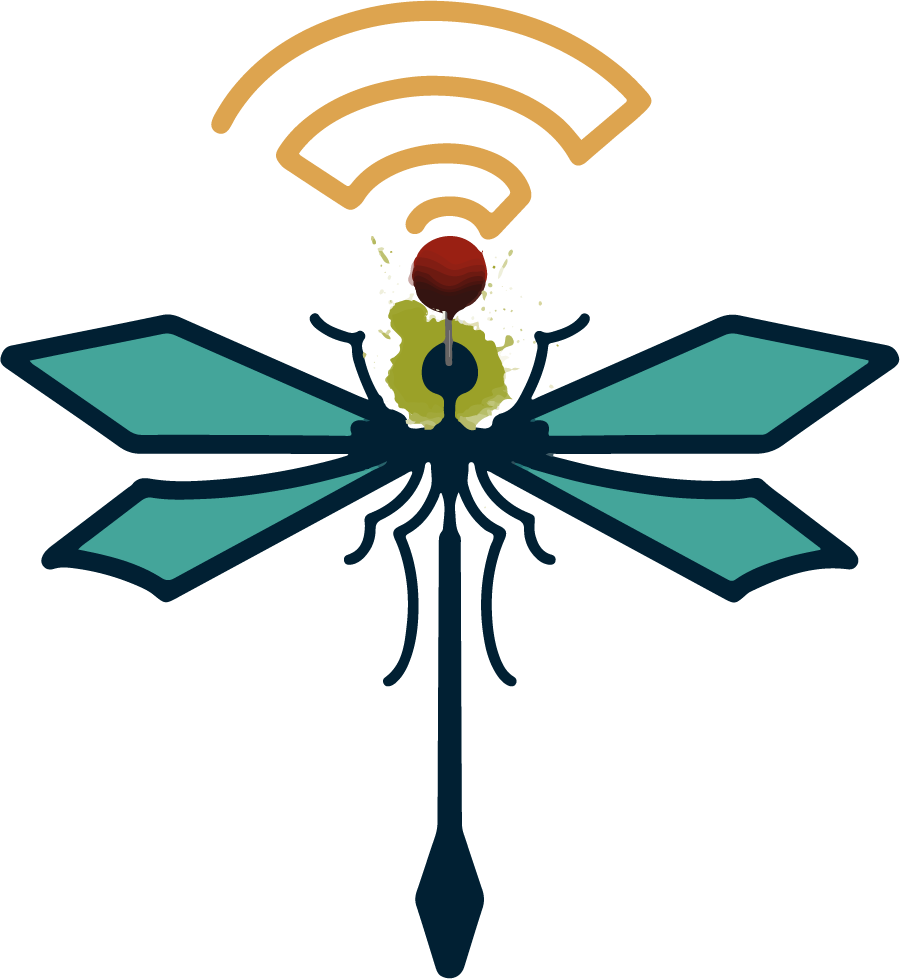
\includegraphics[width=2cm,keepaspectratio]{dragonblood.png}%
  }\fi} % replace with your own command


\colorlet{punct}{red!60!black}
\definecolor{background}{HTML}{EEEEEE}
\subject{COM-506 presentation}
\definecolor{delim}{RGB}{20,105,176}
\colorlet{numb}{magenta!60!black}

\lstdefinelanguage{json}{
    basicstyle=\normalfont\ttfamily,
    numbers=left,
    numberstyle=\scriptsize,
    stepnumber=1,
    numbersep=8pt,
    showstringspaces=false,
    breaklines=true,
    frame=lines,
    backgroundcolor=\color{background},
    literate=
     *{0}{{{\color{numb}0}}}{1}
      {1}{{{\color{numb}1}}}{1}
      {2}{{{\color{numb}2}}}{1}
      {3}{{{\color{numb}3}}}{1}
      {4}{{{\color{numb}4}}}{1}
      {5}{{{\color{numb}5}}}{1}
      {6}{{{\color{numb}6}}}{1}
      {7}{{{\color{numb}7}}}{1}
      {8}{{{\color{numb}8}}}{1}
      {9}{{{\color{numb}9}}}{1}
      {:}{{{\color{punct}{:}}}}{1}
      {,}{{{\color{punct}{,}}}}{1}
      {\{}{{{\color{delim}{\{}}}}{1}
      {\}}{{{\color{delim}{\}}}}}{1}
      {[}{{{\color{delim}{[}}}}{1}
      {]}{{{\color{delim}{]}}}}{1},
}


%%%%%%%%%%%%%%%%%%%%%%%%%%%%%%%%%%%%%%%%%%%%%%%%%%%%%%%%%%%%%%%%%%%%%
\setcounter{tocdepth}{1}
\begin{document}
\defverbatim[colored]\exampleCode{
\begin{pythoncode}
def hash_to_group(password, mac1, mac2):
        for counter in range(1,256):
            seed = Hash(mac1,mac2,password,counter)
            value = KDF(seed, label, p)
            if value >= p: continue
            Elem = math.pow(value, (p-1)/q) mod p
            if Elem > 1: return Elem
\end{pythoncode}
}


\defverbatim[colored]\exampleCodeB{
\begin{pythoncode}
    seed = Hash(mac1,mac2,password,counter)
    value = KDF(seed, label)
\end{pythoncode}
}

\defverbatim[colored]\exampleCodeC{
\begin{pythoncode}
def hash_to_curve(password, mac1, mac2):
        k = 40, found = False
        while count < k:
            count++
            seed = Hash(mac1,mac2,password,count)
            value = KDF(seed, label, p)
            if value >= p: continue
            if quad_res(value^3 + a * value + b, p):
                if not found:
                    x,found = value, True
                    password = rand()
        y = sqrt(x^3+a*x+b) mod p
        return (x,y)
\end{pythoncode}
}

\defverbatim[colored]\exampleCodeD{
\begin{pythoncode}
            if value >= p: continue
            if quad_res(value^3 + a * value + b, p):
                ...
\end{pythoncode}
}


\defverbatim[colored]\exampleCodeE{
\begin{pythoncode}
def hash_to_curve(password, mac1, mac2):
        k = 40
        while count < k:
            seed = Hash(mac1,mac2,password,count)
            value = KDF(seed, label, p)
            ...
            if quad_res(value^3 + a * value + b, p):
               ...
        y = sqrt(x^3+a*x+b) mod p
        ...
\end{pythoncode}
}

\begin{frame}
  \titlepage
\end{frame}

\placelogofalse
\begin{frame}{Outline}
  \tableofcontents
  % possibilité d'ajouter l'option [pausesections]
\end{frame}

\section{Short History of IEEE 802.11 (WLAN) security}
\placelogofalse
\begin{frame}{IEEE 802.11 history}
\begin{figure}
    \centering
\tikzset{every picture/.style={line width=0.75pt}} %set default line width to 0.75pt        

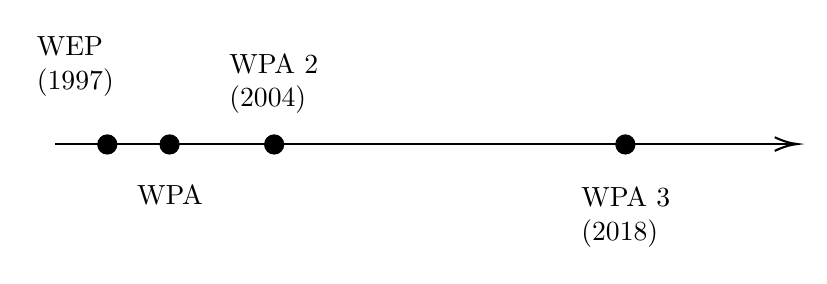
\begin{tikzpicture}[x=0.75pt,y=0.75pt,yscale=-1,xscale=1]
%uncomment if require: \path (0,300); %set diagram left start at 0, and has height of 300

%Straight Lines [id:da342576557268067] 
\draw    (100,125) -- (455.5,125) ;
\draw [shift={(457.5,125)}, rotate = 180] [color={rgb, 255:red, 0; green, 0; blue, 0 }  ][line width=0.75]    (10.93,-3.29) .. controls (6.95,-1.4) and (3.31,-0.3) .. (0,0) .. controls (3.31,0.3) and (6.95,1.4) .. (10.93,3.29)   ;
%Shape: Circle [id:dp4729841814387499] 
\draw  [fill={rgb, 255:red, 0; green, 0; blue, 0 }  ,fill opacity=1 ] (120.4,125.2) .. controls (120.4,122.66) and (122.46,120.6) .. (125,120.6) .. controls (127.54,120.6) and (129.6,122.66) .. (129.6,125.2) .. controls (129.6,127.74) and (127.54,129.8) .. (125,129.8) .. controls (122.46,129.8) and (120.4,127.74) .. (120.4,125.2) -- cycle ;
%Shape: Circle [id:dp7735969428476019] 
\draw  [fill={rgb, 255:red, 0; green, 0; blue, 0 }  ,fill opacity=1 ] (150.4,125.2) .. controls (150.4,122.66) and (152.46,120.6) .. (155,120.6) .. controls (157.54,120.6) and (159.6,122.66) .. (159.6,125.2) .. controls (159.6,127.74) and (157.54,129.8) .. (155,129.8) .. controls (152.46,129.8) and (150.4,127.74) .. (150.4,125.2) -- cycle ;
%Shape: Circle [id:dp4256196026615977] 
\draw  [fill={rgb, 255:red, 0; green, 0; blue, 0 }  ,fill opacity=1 ] (200.8,125.2) .. controls (200.8,122.66) and (202.86,120.6) .. (205.4,120.6) .. controls (207.94,120.6) and (210,122.66) .. (210,125.2) .. controls (210,127.74) and (207.94,129.8) .. (205.4,129.8) .. controls (202.86,129.8) and (200.8,127.74) .. (200.8,125.2) -- cycle ;
%Shape: Circle [id:dp025651477508852993] 
\draw  [fill={rgb, 255:red, 0; green, 0; blue, 0 }  ,fill opacity=1 ] (370,125.2) .. controls (370,122.66) and (372.06,120.6) .. (374.6,120.6) .. controls (377.14,120.6) and (379.2,122.66) .. (379.2,125.2) .. controls (379.2,127.74) and (377.14,129.8) .. (374.6,129.8) .. controls (372.06,129.8) and (370,127.74) .. (370,125.2) -- cycle ;

% Text Node
\draw (109.6,87.6) node   [align=left] {WEP\\(1997)};
% Text Node
\draw (155.2,149.6) node   [align=left] {WPA};
% Text Node
\draw (205.2,96) node   [align=left] {WPA 2\\(2004)};
% Text Node
\draw (374.8,160.4) node   [align=left] {WPA 3\\(2018)};


\end{tikzpicture}
    \label{fig:my_label}
\end{figure}    



\begin{columns}
\begin{column}{0.3\textwidth}
   \begin{block}{WEP}
   \begin{itemize}
       \item relies on the RC4 cipher
       \item 104 bit key
       \item FMS attack
       \item passive key recovery
   \end{itemize}
   \end{block}
   \vfill
\end{column}
\begin{column}{0.3\textwidth}  %%<--- here
    \begin{block}{WPA}
    \begin{itemize}
        \item Temporal Key Integrity Protocol (TKIP)
        \item Key mixing function
        \item 64 bit MAC
        \item still relies on RC4
    \end{itemize}
   \end{block}
\end{column}
\begin{column}{0.3\textwidth}
    \begin{block}{WPA2}
        \begin{itemize}
   \item Mandatory support for AES-CCMP
    \item Four way handshake
   \item WPA2-PSK vulnerable to offline bruteforce attacks
   \item KRACK attacks (\cite{vanhoef-ccs2017})
   \end{itemize}
   \end{block}
\end{column}
\end{columns}
\end{frame}
\placelogofalse
\begin{frame}{WPA3: The sucessor of WPA2}
\begin{figure}[H]
    \centering
    
\includegraphics[width=0.5\textwidth]{images/wpa3.png}
    \label{fig:my_label}
\end{figure}
    \begin{exampleblock}{Protection against offline bruteforce attacks}
WPA2-PSK remplaced by WPA3-SAE (variant of the \textit{Dragonfly} protocol).
\end{exampleblock}
\begin{columns}
\begin{column}{0.6\textwidth}  %%<--- here

\begin{itemize}
    \item 192 bit security for entrepise networks
    \item Opportunistic wireless encryption (OWE) for open networks
    \item Modern primitive support (AES-GCM, EC support)
\end{itemize}
\end{column}
\begin{column}{0.4\textwidth}
    \begin{itemize}
        \item Simplified setup for display-less devices

    \end{itemize}
\end{column}
\end{columns}


\end{frame}
\placelogofalse
\section{The SAE protocol (dragonfly variant)}
\begin{frame}{SAE: Simultanous Authentication of Equals}
    \begin{itemize}
        \item Password authenticated key exchange (PAKE)
        \item Supports ECP and MODP groups
        \item Standart run consists of 3 phases:
        \begin{enumerate}
            \item Password derivation
            \item Commit phase
            \item Confirm phase
        \end{enumerate}
    \end{itemize}
    \vfill
We will now go through the commit and confirm phases.
\end{frame}
\begin{frame}{SAE handshake}
Assume both parties used the shared password $p_s$ to derive a point $P$ on an agreed EC.
\begin{figure}
    \centering
    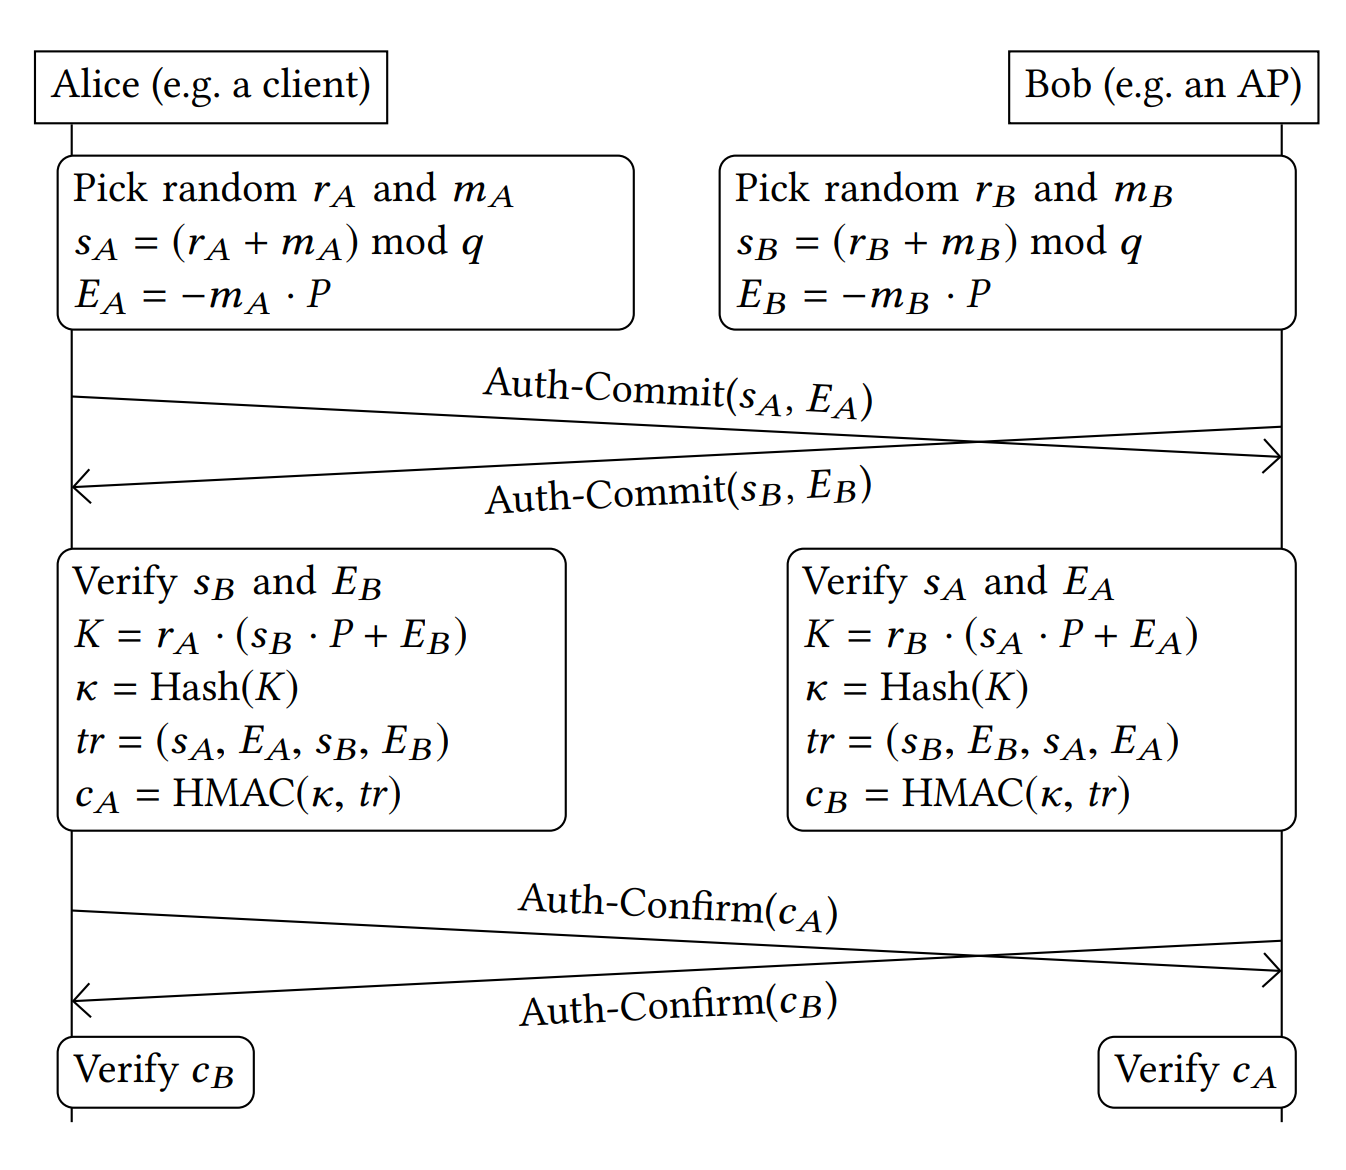
\includegraphics[width=0.6\textwidth]{sae_handshake.png}
    \caption{SAE handshake (taken from \cite{vanhoef-sp2020-dragonblood})}
    \label{fig:my_label}
\end{figure}
\end{frame}
\section{The Dragonblood attacks}
\begin{frame}{Dragonblood}

\begin{columns}
\begin{column}{0.6\textwidth}  %%<--- here
Downgrade attacks:
\begin{itemize}
    \item Downgrade of the group parameters used in SAE
    \item Downgrade attack agains WPA3 transition mode
\end{itemize}
Weaknesses in the dragonfly handshake:
\begin{itemize}
    \item Timing-based side channel attack
    \item Cache-based side channel attack
    \item Denial of Service attack
\end{itemize}
\end{column}
\begin{column}{0.4\textwidth}
    \begin{figure}
        \centering
        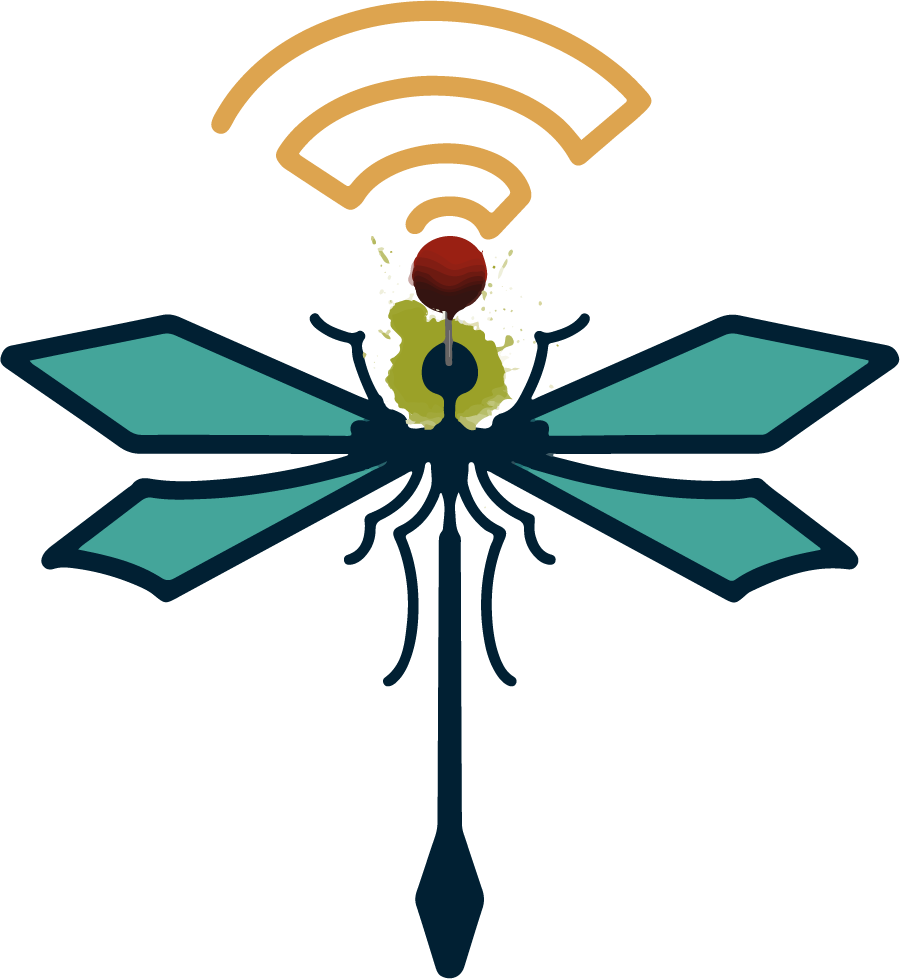
\includegraphics[width=0.5\textwidth]{dragonblood.png}
        \label{fig:my_label}
    \end{figure}
\end{column}
\end{columns}
    
\end{frame}
\begin{frame}{Password derivation: Hash to MODP}
\begin{figure}
    \centering
    \exampleCode
    \caption{(simplified) hash2modp function}
    \label{fig:my_label}
\end{figure}
\begin{itemize}
    \pause
    \item Number of iteration depends on password !
    \pause 
    \item Number of iterations also depends on mac values!
\end{itemize}
\end{frame}
\begin{frame}{More subtle timing leaks}
    The line
    \begin{verbatim}
        if value >= p: continue
    \end{verbatim}
    Also induces a timing leak. Given a MODP group we can compute the probability that the KDF returns an invalid output. \vspace{30pt}
    \begin{itemize}
        \item We will come back to this in a few slides. This leak is more pronounced for certain elliptic curves.
    \end{itemize}
\end{frame}


\begin{frame}{How can we deduce the password?}
    Imagine we have a list of passwords:
    \begin{itemize}
        \item \texttt{pass123} \hfill Simulated number of iterations: 4 | Actual iterations: 3
        \item \texttt{password} \hfill Simulated number of iterations: 2 | Actual iterations: 5
        \item \texttt{r0ckstar} \hfill Simulated number of iterations: 1 | Actual iterations: 1
        \item \texttt{asdfg} \hfill Simulated number of iterations: 2 | Actual iterations: 2
        \item ...
    \end{itemize}
    \vspace{30pt}
    \textit{ \Large{What is the valid password ?}}
\end{frame}
\begin{frame}{How can we deduce the password?}
    Imagine we have a list of passwords:

    \begin{itemize}
        \item \st{\texttt{pass123}} \hfill Simulated number of iterations: \textcolor{red}{4} | Actual iterations: \textcolor{red}{3}
        \item \st{\texttt{password}} \hfill Simulated number of iterations: \textcolor{red}{2} | Actual iterations: \textcolor{red}{5}
        \item \texttt{r0ckstar} \hfill Simulated number of iterations: 1 | Actual iterations: 1
        \item \texttt{asdfg} \hfill Simulated number of iterations: 2 | Actual iterations: 2
        \item ...
    \end{itemize}
        \vspace{30pt}
        \textit{ \Large{Do we have any other information which might help us exclude further passwords ?}}
\end{frame}
\begin{frame}{Additional information: Spoofing MAC addresses}
    \exampleCodeB
    We can spoof MAC addresses
    \begin{itemize}
        \item \texttt{r0ckstar} \hfill sim. #iter with MAC $M_1$: 1 | Actual iterations: 1
        \item \st{\texttt{r0ckstar}} \hfill sim. #iter with MAC $M_2$: \textcolor{red}{1} | Actual iterations: \textcolor{red}{2}

        \item \texttt{asdfg} \hfill Simulated number of iterations: 2 | Actual iterations: 2
        \item ...
    \end{itemize}
        \vspace{30pt}
        \textit{ \Large{What about EC based crypto ?}}
\end{frame}
\begin{frame}{Hash2Curve}
\begin{figure}
    \centering
\exampleCodeC
\caption{(Simpified) Hash2Curve pseudocode}
    \label{fig:my_label}
\end{figure}
    \Large{\textit{What are the key differences compared to} \texttt{hash2modp} ?}
\end{frame}
\begin{frame}{Quardratic residues and blinding}
    We say that $x^3+ax+b$ is a quadratic residue $\mod p$ if $\exists e$ s.t
    $$x^3+ax+b \equiv e^2 \mod p$$
    recall the ECs are defined by the Weierstrass equation
    $$y^2 = x^3 + ax + b \mod p$$
    To prevent timing leaks by \texttt{quad\_res} we compute the existence of a quadratic residue of
    $$(x^3+ax+b)r^2n$$
    where $r$ is a random number and $n$ is a random quadratic non-residue.
\end{frame}
\begin{frame}{Timing leaks for Brainpool curves}
\exampleCodeD

\begin{columns}
\begin{column}{0.6\textwidth}  %%<--- here
\begin{table}[]
\begin{tabular}{@{}lll@{}}
\toprule
Curve           & len(p) & $\mathbb{P}[value \geq p]$ \\ \midrule
brainpoolP224r1 & 224    & 15.72 \%                   \\
brainpoolP256r1 & 256    & 33.60 \%                   \\
brainpoolP384r1 & 384    & 45.03 \%                   \\
brainpoolP512r1 & 512    & 33.26 \%                   \\ \bottomrule
\end{tabular}
\end{table}
\end{column}
\begin{column}{0.4\textwidth}
\begin{itemize}
    \item Extra iterations depend on random password
    \item More iterations done on the real password implies lower execution time variance
    \item Non trivial to exploit
\end{itemize}    
\end{column}
\end{columns}
\vspace{30pt}
\textit{\Large{What makes brainpool curves so "bad" ?}}
\end{frame}
\begin{frame}{Timing leaks for brainpool curves}
    The KDF returns a random stream of $n$ bits with $n$ being the number of bits needed to represent $p$.
    \begin{columns}
\begin{column}{0.6\textwidth}  %%<--- here
A simple example:
\begin{itemize}
    \item Take $p = 17 (=0b10001)$
    \item The KDF returns $5$ bits
    \item What is the probability that $\text{KDF}(\cdot) \geq p$ ?
    $$ 2^{-5} \left( \sum_{i=0}^3 {3 \choose i}\right) = 0.25$$
    \item What about $p = 31$ ?
    \item $31$ is a \textit{Mersenne prime}: 31 = $2^5-1$
    \item We also need 5 bits to represent 31 ($0b11111$).
    \item But now $\mathbb{P}[$\text{KDF}(\cdot) \geq p$] \approx 0.031$
\end{itemize}
\end{column}
\begin{column}{0.4\textwidth}
\begin{itemize}
    \item Brainpool curves use \textit{random} primes.
    \item In contrast, NIST curves use quasi Mersenne primes, for example
    $$p_{192} = 2^{192}  - 2^{64}  - 1$$
    or
    $$p_{521} = 2^{521}  - 1 $$
\end{itemize}
\begin{exampleblock}{Conclusion}
This results in very low probabilities for invalid KDF values compared to the case of random brainpool primes.
\end{exampleblock}

\end{column}
\end{columns}
\end{frame}
\begin{frame}{Exploiting timing leaks in practice}
\textit{Can we actually deduce the number of iterations ?}
\begin{figure}
    \centering
    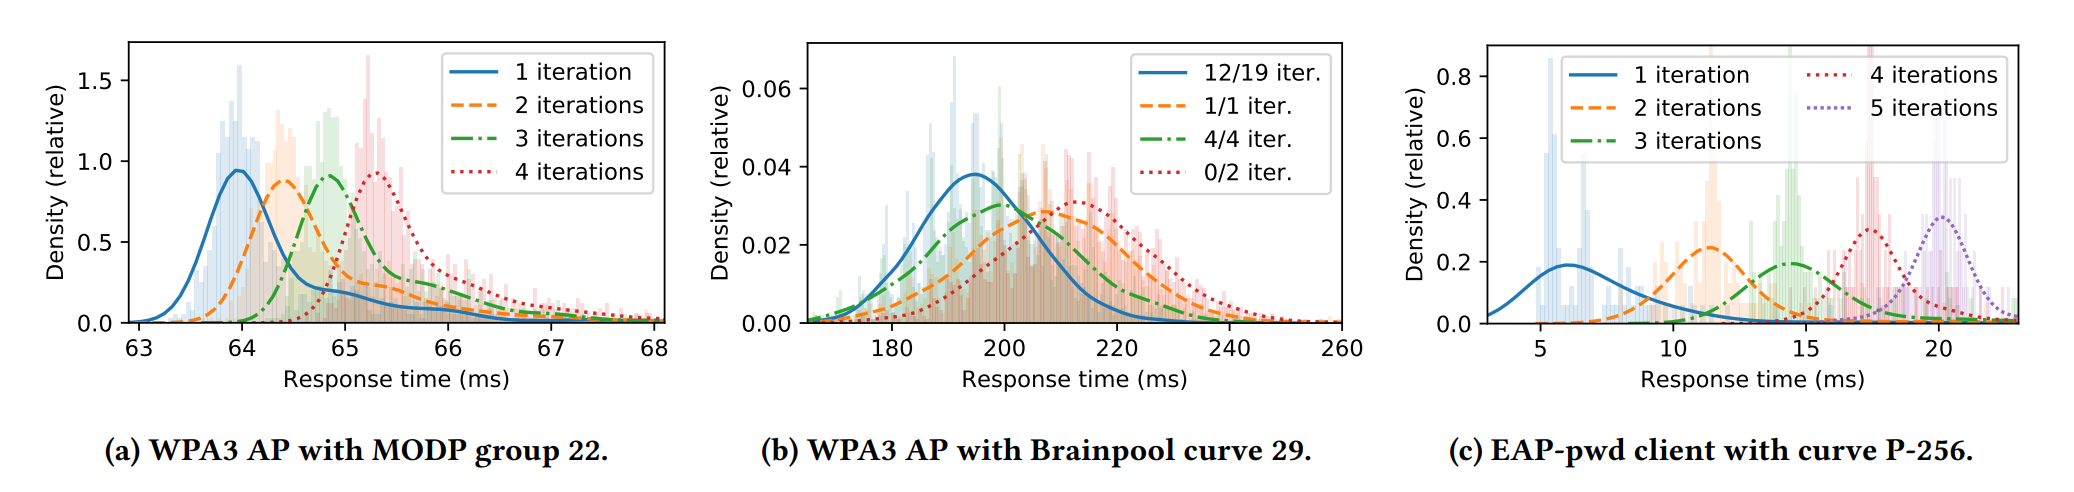
\includegraphics[width=1\textwidth]{dragonflytiming.png}
    \caption{Response time distributions (\cite{vanhoef-sp2020-dragonblood})}
    \label{fig:my_label}
\end{figure}
\begin{itemize}
    \item MODP groups: \texttildelow 75 measurements / address
    \item Brainpool: \texttildelow 2000 measurements / address
\end{itemize}
\end{frame}
\begin{frame}{Computational Costs in practice}
Costs are based on an Amazon EC2 P3 instance with 8 V100 GPUs (74\$ / h) 
\vspace{30pt}

\begin{table}[]
\begin{tabular}{llll}
\hline
Wordlist / method    & Size  & Cost for MODP (\$) & Cost for P-256 (\$) \\ \hline
RockYou              &  \texttildelow $10^7$ & $2.1 \cdot 10^{-6}$   & $4.4 \cdot 10^{-4}$      \\
HaveIBeenPwned       & \texttildelow $10^8$  & $8.0 \cdot 10^{-5}$      & $1.7 \cdot 10^{-2}$     \\
Probable wordlist    & \texttildelow $10^9$ & $1.2 \cdot 10^{-3}$    & $2.5 \cdot 10^{-1}$     \\ \hline
Bruteforce 8 symbols & \texttildelow $10^{14}$ & $670$           & $14'000$          \\ \hline
\end{tabular}
\cation{Estimated costs (\cite{vanhoef-sp2020-dragonblood})}
\end{table}
\end{frame}
\begin{frame}{Denial of service attacks}
    \exampleCodeE
    \begin{itemize}
        \item Defenses (extra iterations, QR blinding) are costly
        \item Tradeoff between DoS and timing leak resistance
        \item Defense mechanism: Cookies (similar to IKEv2 and wireguard)
        \item Problem: Wifi is a broadcast medium, we can steal and reflect cookies.
        \item At 7 faked commits per second the AP is at 80\% CPU usage (500bit EC)
    \end{itemize}
\end{frame}
\begin{frame}{Denial of service attacks}
    \begin{figure}
        \centering
        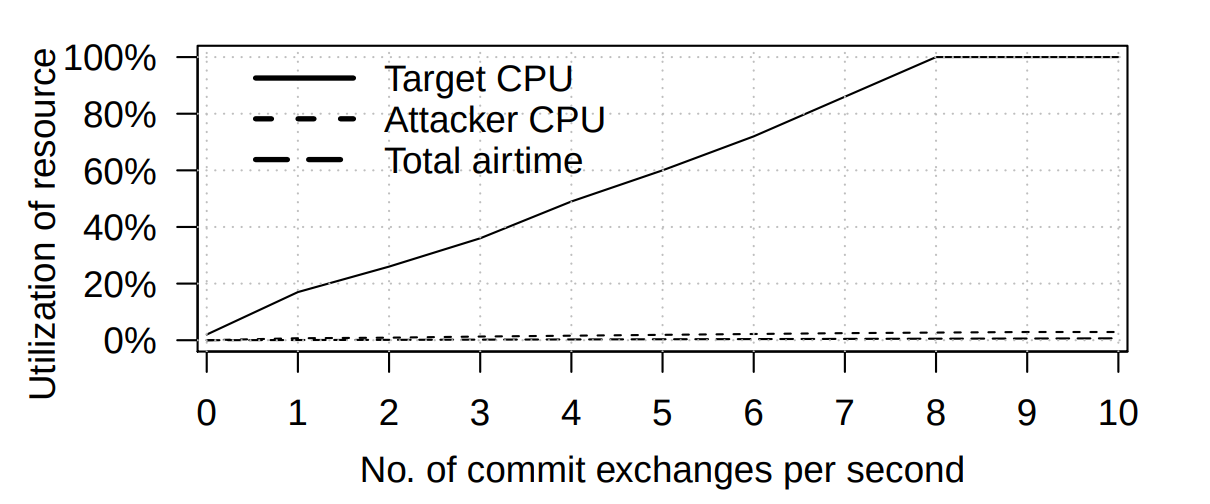
\includegraphics[width=0.7\textwidth]{dos.png}
        \caption{DoS attack against an AP using a P521 curve (\cite{vanhoef-sp2020-dragonblood})}
        \label{fig:my_label}
    \end{figure}
    \begin{itemize}
        \item Implemented side channel defenses are too costly
        \item Low end devices might choose not to implement them, favouring performance
    \end{itemize}
\end{frame}
\begin{frame}{Crypto Downgrade attacks}
    Semantic: Parameters are proposed by client, server responds with Yes/No
    \begin{figure}
        \centering
        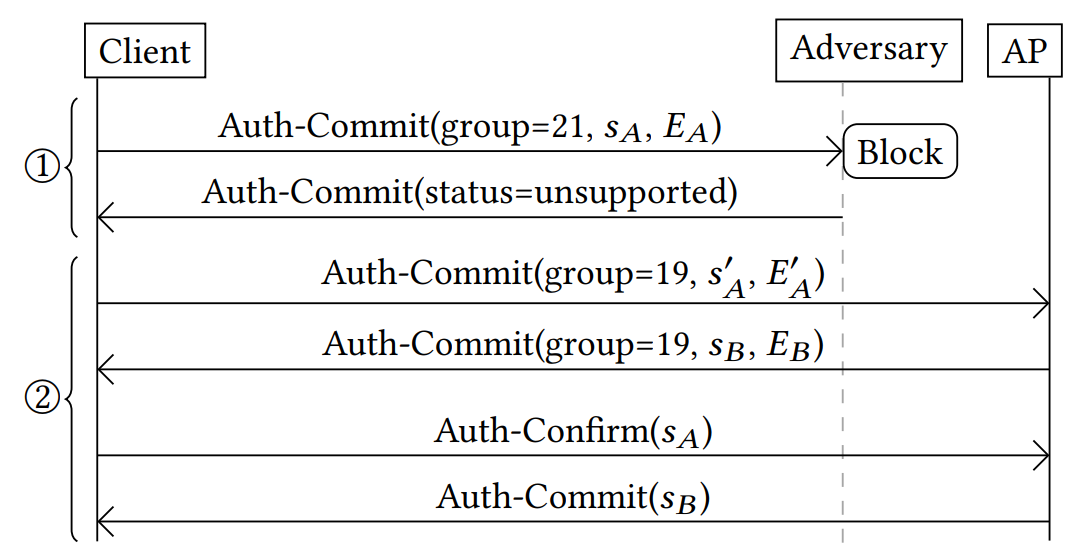
\includegraphics[width=0.7\textwidth]{downgrade.png}
        \caption{SAE group negotiation (\cite{vanhoef-sp2020-dragonblood})}
        \label{fig:my_label}
    \end{figure}

    \begin{exampleblock}{Solution}
    Only support known good groups and curves 
    \end{exampleblock}
\end{frame}
\begin{frame}{WPA3-transition mode}
    WPA3 transition mode dictates that an AP accepts WPA2 and WPA3 connections using the same password.
    \begin{itemize}
        \item An attacker cannot: Trick a client that an AP in WPA3 transition mode only supports WPA2
    \end{itemize}
   \begin{figure}
       \centering
       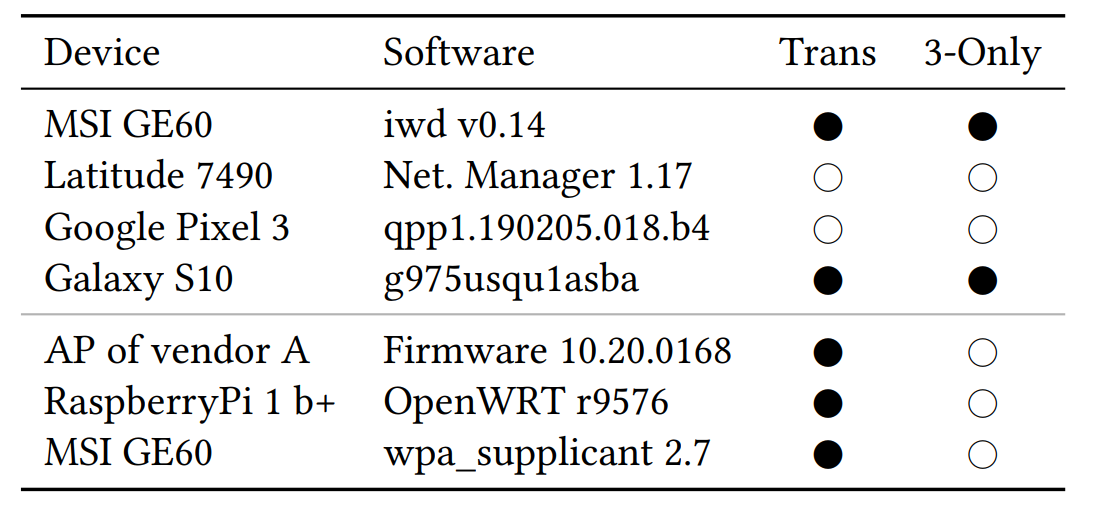
\includegraphics[width=0.5\textwidth]{wpa3_downgrade.png}
       \caption{List of devices vulnerable to WPA3-trans. / WPA 3 downgrade attacks (\cite{vanhoef-sp2020-dragonblood})}
       \label{fig:my_label}
   \end{figure}
    \begin{itemize}
        \item Setup a rogue WPA2 AP with the same SSID close to the target
        \item Perform a partial handshake (until client sends authenticated packet)
    \end{itemize}
    \begin{exampleblock}{Solution}
    Remember which networks support WPA3 (trust on first use)
    \end{exampleblock}
\end{frame}
\begin{frame}{Invalid Curve attack}
\begin{figure}
    \centering
   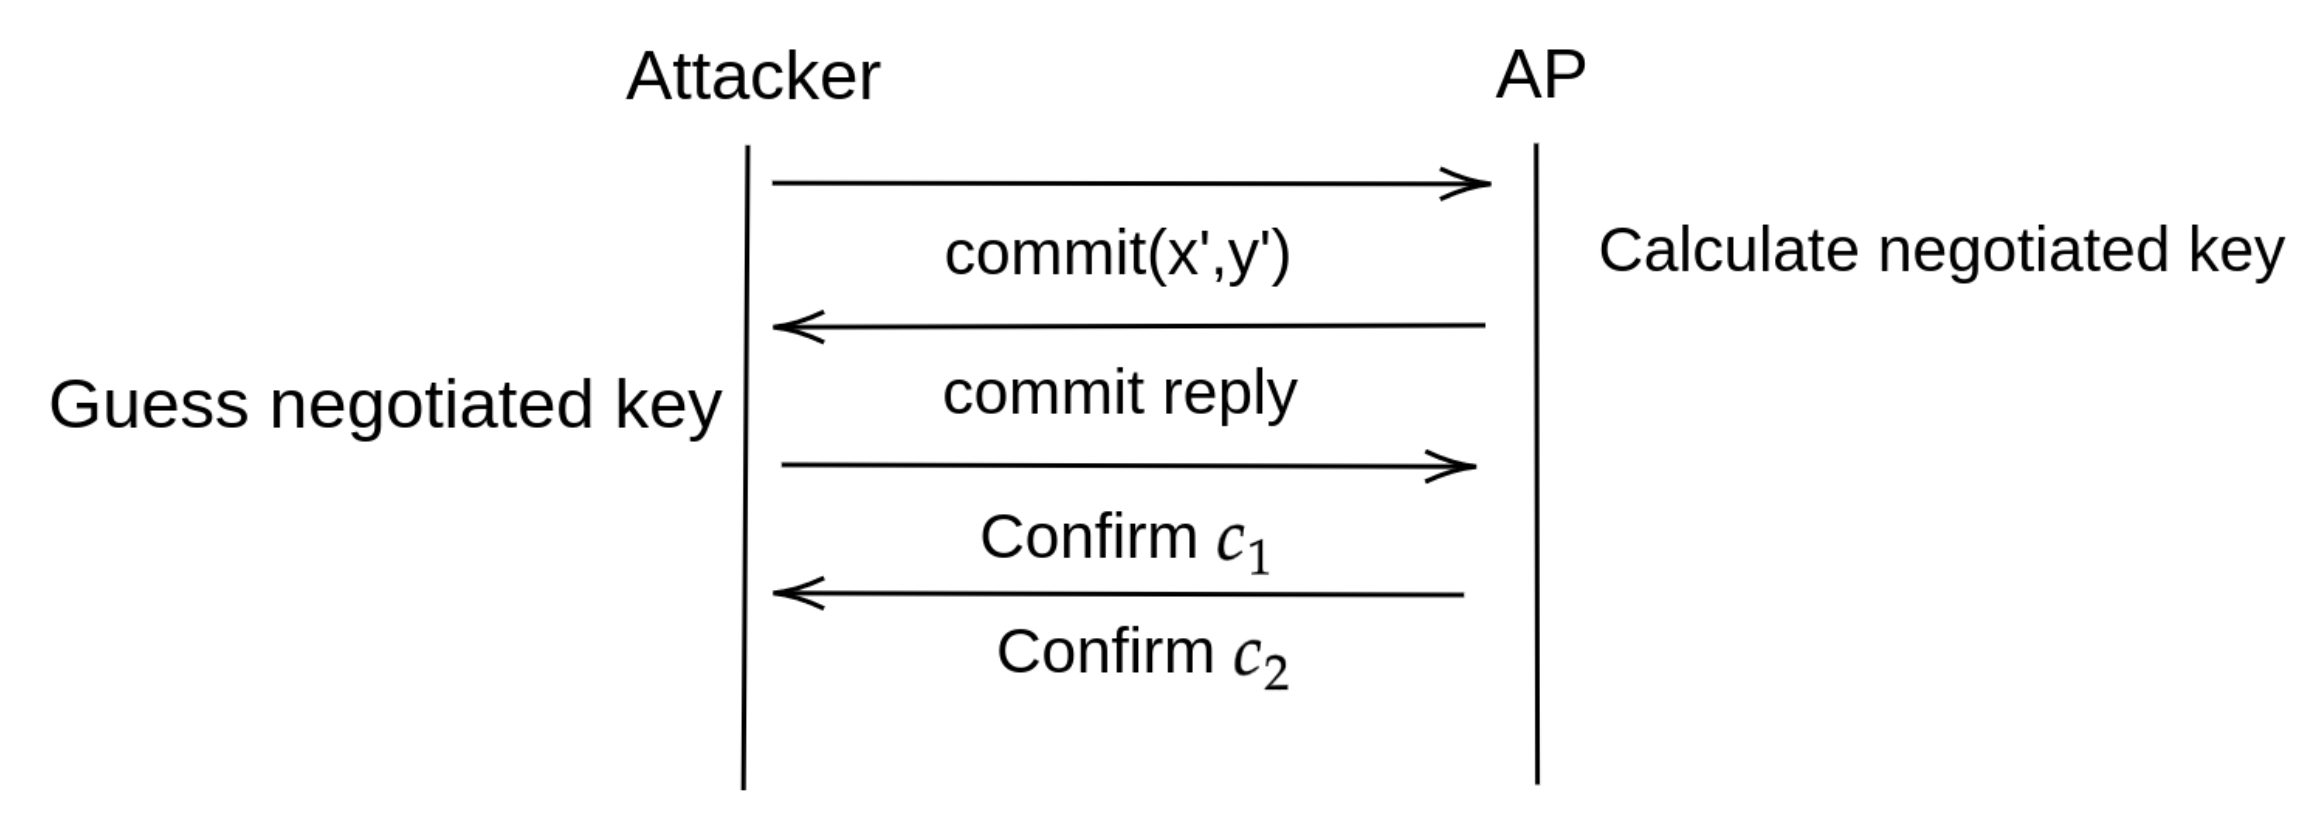
\includegraphics[width=1\textwidth]{invalidcurve.png}
    \caption{Forcing the AP to use an invalid point makes the negotiated key predictable}
    \label{fig:my_label}
\end{figure}
\begin{exampleblock}{Solution}
Implementation should check whether the point is valid (on the curve)
\end{exampleblock}
\end{frame}
\begin{frame}{Reflection attack (EAP-PWD)}
    \begin{itemize}
        \item On EAP-PWD, the dragonfly handshake is initialized by the AP
        \item An Attacker can reflect the received frames
    \end{itemize}
    \begin{figure}
        \centering
        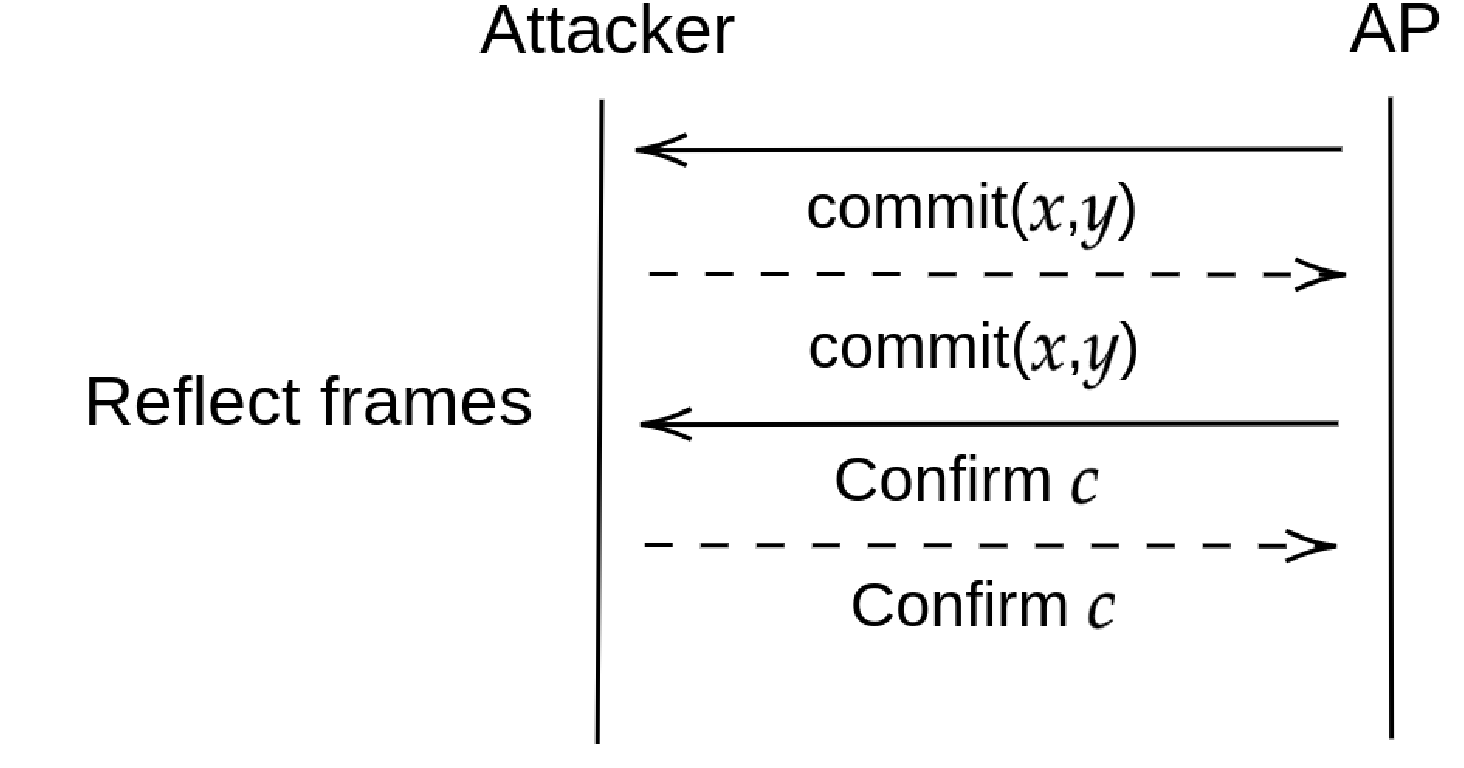
\includegraphics[width=0.7\textwidth]{reflect.png}
        \caption{Reflection attack in a EAP-PWD scenario}
        \label{fig:my_label}
    \end{figure}
    \textit{\large{Is the attacker authenticated ? Can he send traffic ?}}
\end{frame}
\begin{frame}{Summary: Implementation vulnerabilities}
    \begin{figure}
        \centering
        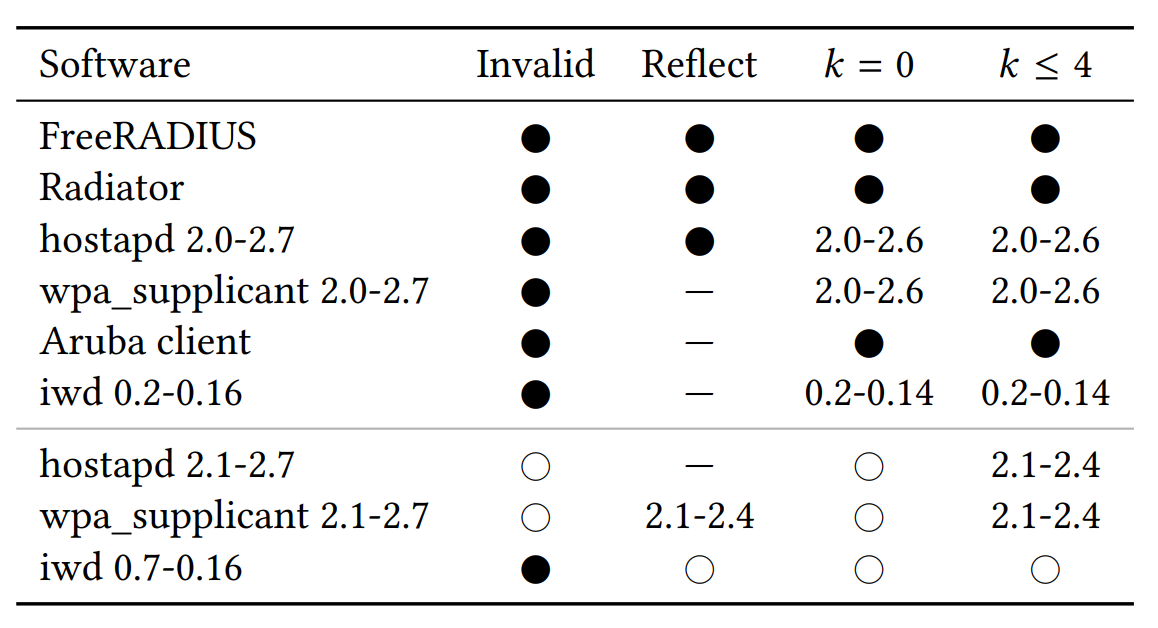
\includegraphics[width=0.7\textwidth]{summary.png}
        \caption{Overview of SAE (bottom) / EAP-PWD (top) implementation vulnerabilities (\cite{vanhoef-sp2020-dragonblood})}
        \label{fig:my_label}
    \end{figure}
\end{frame}
\section{Conclusion}
\begin{frame}{Conclusion}
    Today we've seen:

\begin{itemize}
    \item Multiple side channel attacks
    \item The cost of mitigating side channel attacks
    \item Multiple implementation specific vulnerabilities
\end{itemize}
You can find the slides / tex online at my GitHub
\begin{figure}[H]
    \centering
    
\includegraphics[width=0.2\textwidth]{frame.png}
    \label{fig:my_label}
\end{figure}
 \begin{exampleblock}{Should I use WPA3?}
 Yes. Patches are on the way. Even without them, WPA3 offers better security than WPA2.
 \end{exampleblock}
\end{frame}
\begin{frame}[allowframebreaks]
        \frametitle{References}
        \printbibliography
\end{frame}
\end{document}
